
 
% Diese Zeile bitte -nicht- aendern.
 \documentclass[course=erap]{aspdoc}
 \usepackage{tikz}
 \usepackage{graphicx}
 \usepackage[export]{adjustbox}
 \usepackage{amssymb}
 %%%%%%%%%%%%%%%%%%%%%%%%%%%%%%%%%
 %% TODO: Ersetzen Sie in den folgenden Zeilen die entsprechenden -Texte-
 %% mit den richtigen Werten.
 \newcommand{\theGroup}{team175} % Beispiel: 42
 \newcommand{\theNumber}{A316} % Beispiel: A123
 \author{Hans Preinfalk \and Viktor Bayo \and Georgy Chomakhashvili}
 \date{Sommersemester 2022} % Beispiel: Wintersemester 2019/20
 %%%%%%%%%%%%%%%%%%%%%%%%%%%%%%%%%
 % Diese Zeile bitte -nicht- aendern.
 \title{Gruppe \theGroup{} -- Abgabe zu Aufgabe \theNumber}
 
 \begin{document}

 \maketitle
 
 \section{Einleitung}
 
 
Die vorliegende Arbeit, die im Rahmen des Grundlagenpraktikums der Rechnerarchitektur durchgeführt wurde, behandelt die Approximation der Areasinus Hyperbolicus Funktion (arsinh), der Umkehrfunktion des Sinus Hyperbolicus (sinh) und die Analyse der implementierten Berechnungen. Zuerst werden die Problemstellung sowie die Eigenschaften der zu betrachtenden Funktion beschrieben. Im Weiteren erfolgt die Darstellung des Lösungsansatzes, welche die mathematische Herleitungen sowohl der reinen Reihendarstellung als auch der Lookup-Tabellen beinhaltet. Dann werden die Implementierungen auf Genauigkeit und Laufzeit geprüft. Schließlich folgt die Zusammenfassung mit einem Fazit.

Die aktuelle Problematik der zuvor beschriebenen Funktion lässt sich in die Bereiche Konzeption (theoretisch) und Implementierung (praktisch) aufteilen.

Der theoretische Teil impliziert die mathematische Herleitung, anhand welcher eine Formel für die Approximation von arsinh als Reihendarstellung und die Logik für die Methode der Suchtabellen erstellt werden soll.

Der praktische Teil der Problematik besteht darin, die Wahl zwischen den beiden möglichst performanten und möglichst genauen Implementierungen der zuvor beschriebenen Funktion zu ermöglichen. Allerdings gibt es eine wichtige Bedingung, die besagt, dass der Code auf nicht komplexe Operationen, wie zum Beispiel die vier Grundrechenarten, basieren muss. Es sollte auch möglich sein, eine der Implementierungen auszuwählen und die Laufzeit der unterschiedlichen Implementierungen vergleichen zu können. Es gibt jedoch eine Vergleichsimplementierung, die komplexere Rechenoperationen verwenden darf.

Um das Konzept der Funktionsapproximation nachvollziehen zu können, ist es erforderlich, zuerst auf die Eigenschaften der Funktion an sich einzugehen. arsinh ist eine inverse Funktion zum hyperbolischen Sinus $(x = \text{sinh}(y))$, die einen Definitionsbereich $]-\infty;+\infty[$ und einen Wertebereich $]-\infty;+\infty[$ hat. Die Funktion ist punktsymmetrisch zum Ursprung und streng monoton steigend. Zudem ist sie an der $y$-Achse gespiegelt.

Die hyperbolische Areasinus Funktion lässt sich folgendermaßen darstellen: 
\begin{equation}\label{func}
    \text{arsinh}(x) = \ln(x + \sqrt{x^2 + 1}) \ \ \ \text{mit} \ x \in \mathbb{R}
\end{equation}

Wobei für die Asymptote gilt:
\begin{equation}\label{asympt}
    f(x) \rightarrow \pm \ln(2|x|) \ \ \ \text{für} \ x \rightarrow \pm \infty
\end{equation}

Die abgleitete Funktion ist dann:
\begin{equation}\label{ableit}
    \frac{d}{dx} \ \text{arsinh}(x) = \frac{1}{\sqrt{x^2 + 1}}
\end{equation}

Intuitiv ist dann auch der Zusammenhang der arsinh-Funktion mit arcosh anhand der Signumfunktion und des richtigen Einsetzens von x in arcosh, welcher sich durch die Multiplikation von $\text{sgn}(x)$ mit $\text{arcosh}(\sqrt{x^2 + 1})$ ergibt.
 \section{Lösungsansatz}
 \subsection{Einlesen der Befehle anhand des Rahmenprogramms}
 
     Das Rahmenprogramm wurde entsprechend der Aufgabenstellung entwickelt. Das Programm realisiert folgende Befehle: $-V<int> $, $-B<int>$,$<float>$,$-h$,$--help$. Um die inkorrekte Eingabe der optionalen Argumenten für die ersten zwei Befehle zu vermeiden, wird es überprüft, ob dies eine gültige Zahl ist. Als eine gültige Zahl für die Option wird diese dann behandelt, falls sie $\geq 0$ ist, da es keine negativen Optionen für die Implementierung und keine negative Anzahl an Wiederholungen gibt, und einem Integer entspricht, also nicht dezimal und kleiner-oder-gleich dem Maximum dieses Datentyps ist. Bei dem ersten Befehl werden nur $0,1,2$ oder keine Zahl akzeptiert, da es nur drei Implementierungen gibt. Als Hauptimplementierung wurde die Reihendarstellung gewählt, da diese die genauesten Werte liefert. Die Laufzeit wird anhand einer in der Kommandozeile im Voraus gewählten Implementierung gemessen. In dem Fall, dass die Implementierung vor diesem Befehl nicht gewählt wurde, wird die Laufzeit von der Hauptimplementierung gemessen. 
     
     In dem Programm wird auch der Fall betrachtet, bei dem die Befehle die Standardwerte liefern. Wenn keine Implementierung gewählt wurde, wird die Hauptimplementierung ausgeführt. Es wird bei der Laufzeitberechnung zwar eine Anzahl an Wiederholungen erwartet, aber es wird auch problemlos ohne ein optionales Argument funktionieren, indem die Laufzeit nur für einen einzigen Funktionsaufruf gemessen wird. Bei fehlender Zahleingabe wird $0$ als Standardwert genommen. Wenn die Kommandozeile keine Befehle enthält, wird die Ausgabe nach vorher beschriebenen Standarten ausgeführt. 
     Um eine sinnvolle und intuitive Eingabe zu ermöglichen, wird nur eine float-Zahl oder keine (dann wird, wie beschrieben, der Standardwert genutzt) angenommen. Es wird auch überprüft, ob der eingegebene $x$-Wert in dem erwarteten Datentypintervall liegt. 
     
     Das Rahmenprogramm überprüft die Korrektheit der Eingaben und gibt spezifizierte Fehlermeldungen aus, falls es bei dem Input etwas Unzutreffendes auftaucht.
    
    \subsection{Reihendarstellung}
    \subsubsection{Herleitung}
    
    Die Herleitung verlangt das schrittweise Umformen der schon bekannten Formel $\eqref{func}$ für die Umkehrfunktion arsinh in die Reihendarstellung.
    
    Dafür werden wir zuerst das Integral der Ableitung nutzen, was der Funktion selbst gleich ist. Somit ergibt sich:
    
    \begin{equation}
        \text{arsinh}(x) = \ln(x + \sqrt{x^2 + 1}) = \int \frac{dx}{\sqrt{1+x^2}} = \int (1+x^2)^{-\frac{1}{2}} dx
    \end{equation}
    
    Hiermit können wir einen Spezialfall der binomischen Reihe der Funktion $(1+x^2)^{-\frac{1}{2}}$ bemerken. Durch die Regel $(1+x)^{\alpha} = \sum_{k=0}^{\infty} (-1)^k \cdot \binom{\alpha}{k} \cdot x^k$ , wobei hier $\alpha = -\frac{1}{2}$ ist, lässt sich die Formel folgendermaßen darstellen:
    
    \begin{equation}
        \int (1+x^2)^{-\frac{1}{2}} dx = \int \sum_{k=0}^{\infty} (-1)^k \cdot \binom{-\frac{1}{2}}{k} \cdot (x^2)^k
    \end{equation}
 
    Durch die Zersetzung des Binomialkoeffizienten $\binom{\alpha}{k} = \frac{\alpha \cdot (\alpha-1) \cdot \ldots \cdot (\alpha-k+1)}{k!}$ für $|x| < 1$ und durch das weitere Umformen ergibt sich:
    
    \begin{equation}
        \int \sum_{k=0}^{\infty} (-1)^k \cdot \binom{-\frac{1}{2}}{k} \cdot (x^2)^k = \int \sum_{k=0}^{\infty} (-1)^k \cdot \frac{(2k-1)!!}{(2k)!!} \cdot x^2
    \end{equation}
    
    Aus der letzten Formel lässt sich eine Reihendarstellung bilden. Dies geschieht dank der bekannten Taylorreihe. Also sieht dann die Reihendarstellung der Umkehrfunktion arsinh so aus:
    
    \begin{equation}\label{reihe}
        x - \frac{1}{2} \cdot \frac{x^3}{3} + \frac{1 \cdot 3 \cdot x^5}{2 \cdot 4 \cdot 5} - \frac{1 \cdot 3 \cdot 5 \cdot x^5}{2 \cdot 4 \cdot 6 \cdot 7} + \ldots + (-1)^k \frac{1 \cdot 3 \cdot 5 \cdot \ldots \cdot (2k -1) \cdot x^{2k + 1}}{2 \cdot 4 \cdot 6 \cdot \ldots \cdot 2k \cdot (2k + 1)} + \dots
    \end{equation}
    
    Diese Reihendarstellung lässt sich in $x \cdot \sum_{k=0}^{\infty} \frac{(2k - 1)!!(-x^2)^k}{(2k)!!(2k+1)}$ verallgemeinern. Dies ist aber nur für $|x| < 1$ gültig. Für den weiteren Verlauf der Funktion wird die Reihendarstellung der Umkehrfunktion arcosh, also $\ln(2x) - \sum_{k=0}^{\infty} \frac{(2k - 1)!!}{(2k) \cdot (2k)!!} \cdot x^{-2k}$, nützlich. Es gilt dann anhand der Relation zwischen zwei hyperbolischen Funktionen Areasinus und Areakosinus \cite{bronshtein2015algebra} und anhand der bekannten Signumfunktion (Vorzeichenfunktion):
    
    \begin{equation}
        \text{arsinh}(x) = (\text{sign}(x)) \ \text{arcosh}(\sqrt{x^2 + 1})
    \end{equation}
 
    Somit lässt sich der Lösungsansatz in zwei Teile aufspalten. Für $|x|<1$ wird arsinh durch die Taylorreihe approximiert. Für $|x|\geq1$ wird die Taylorreihe des Areakosinus Hyperbolicus verwendet. 
    
    \subsubsection{Implementierung}
    
    Zuerst betrachten wir den Fall $|x|<1$. Wie bereits bewiesen wurde, lässt sich die Reihendarstellung hierfür durch die Taylorreihe annähern. Hierzu wird die Formel $\eqref{reihe}$, also auch $x-\frac{1}{2}\cdot \frac{1}{3}\cdot \text{pow}(x,3) +\frac{3}{8}\cdot \frac{1}{5}\cdot \text{pow}(x,5) -\frac{15}{48}\cdot \frac{1}{7}\cdot \text{pow}(x,7) \ldots$ verwendet. Um die Potenzen zu berechnen, wird eine Variable für das Zwischenergebnis bei jeder Iteration zweimal quadriert.
Diese Potenz wird durch eine Zählvariable geteilt, die pro Iteration um zwei inkrementiert wird.
  Der Koeffizient dieser Potenz berechnet sich dadurch, dass eine Zählervariable mit dem Startwert $1$ und eine Nennervariable mit Startwert $2$ pro Iteration mit dem um zwei inkrementierten Wert der Zählervariablen multipliziert wird.
Zuletzt wird das Resultat vom Eingabewert subtrahiert.

 Für $|x|>1$ wird die Taylorreihe der Areakosinus Hyperbolicus Funktion
 verwendet. Aus der mathematischen Herleitung ist es bekannt, dass arcosh$(\text{sqrt}(x\cdot x+1))=$arsinh$(x)$ mit arcosh$(x)= \ln(2x)-(\frac{1}{2}\cdot\frac{1}{x^2}+\frac{3}{8}\cdot\frac{1}{x^4}-\frac{15}{48}\cdot\frac{1}{x^6}\ldots)$. Zunächst wird die Wurzel von $x\cdot x+1$ berechnet, die dann als Eingabewert für die arcosh Funktion dient.
Anschließend wird für $|x|<12$ die Reihendarstellung des Logarithmus berechnet mit $\ln(x)=2*[ \frac{x-1}{x+1} + \frac{1}{3} \cdot \text{pow}(\frac{x-1}{x+1},3) + \frac{1}{5} \cdot \text{pow}(\frac{x-1}{x+1},5)]$. Die Berechnung erfolgt analog zur Berechnung der Taylorreihe von arsinh.

Für $|x|>12$ wird der Logarithmus rekursiv berechnet, indem eine Zählvariable so oft inkrementiert wird und der Eingabewert durch die Basis geteilt wird, bis der Eingabewert kleiner als die Basis ist. Bei Rekursionstiefe 0  stellt die Zählvariable nach Verlassen der Schleife den abgerundeten Logarithmus dar. In dem rekursiven Aufruf wird die Zählvariable
mit dem Ergebnis der restlichen Rekursionsebenen, geteilt durch eins, addiert. In der nächsten Rekursionsebene werden die Parameter, Basis und Eingabewert, vertauscht. Dies geschieht so lange bis der Eingabeparameter $\leq (1.0 + \epsilon)$ ist. Ist das der Fall, wird die Zählvariable zurückgegeben. Dadurch, dass der rekursive Aufruf durch $1.0$ geteilt wird und die Zählvariable $\geq 1$ sein muss, werden ab Rekursionstiefe 1 die Nachkommastellen approximert.
Nach der Berechnung der Asymptote erfolgt auch die Berechnung der Reihendarstellung von arcosh
analog zu der von arcosh. 

Bei negativen Eingabewerten wird lediglich der Eingabewert und das Ergebnis negiert. Der Rest der Berechnung verläuft identisch zu der von positiven Werten.
    
 \subsection{Tabellen Lookup}
 \subsubsection{Herleitung}
    Um die arsinh Funktion mithilfe der Lookup-Tabellen berechnen zu können, braucht man ein Verfahren, bei welchem man die Werte zwischen zwei Messpunkten approximieren kann. Es bieten sich zwar die Polynominterpolation und die logarithmische Interpolation an, werden aber wegen der Ineffizienz zuzüglich verlangsamender Laufzeit durch die Nutzung von komplexeren und zahlreichen Rechenoperationen nicht in Betracht genommen. Die lineare Interpolation hingegen, ist ein möglicher effizienter Lösungsansatz für die Berechnung der Werten von arsinh, der für die vorher beschriebene Problemstellung verwendet werden kann.
    Bei der linearen Interpolation geht es darum, eine Gerade zwischen zwei Punkten zu erstellen und die Werte auf der Geraden als Annäherung zu nehmen.
    
    Die lineare Funktion kann mit der folgenden Formel beschrieben werden: 

    \begin{equation}
        f(x) = m\cdot x + b
    \end{equation}

    Wobei es für die Steigung $m$ und für den $y$-Achsenabschnitt $b$ gilt:
    
    \begin{equation}\label{m}
        m = \frac{f(x_1) - f(x_0)}{x_1 - x_0} 
    \end{equation}
    \begin{equation}\label{b}
        b = f(x_0) - \frac{f(x_1) - f(x_0)}{x_1 - x_0} \cdot x_0
    \end{equation}

    Mit dem Einsetzen von $\eqref{m}$ und $\eqref{b}$ erhält man:
    
    \begin{equation}
        f(x) = \frac{f(x_1) - f(x_0)}{x_1 - x_0} \cdot x + f(x_0) - \frac{f(x_1) - f(x_0)}{x_1 - x_0} \cdot x_0
    \end{equation}
    
    Nach den weiteren Vereinfachungen bekommt man die Formel der linearen Interpolation, nämlich:
    
    \begin{equation}
        f(x) = f(x_0) + \frac{(x - x_0)}{x_1 - x_0} \cdot (f(x_1) - f(x_0))
    \end{equation}
    
    Da arsinh sich für $\lim_{x \to \infty} \text{arsinh}(x) \rightarrow \ln(2|x|)$ mit der Formel $\eqref{asympt}$ immer kleinere Abweichungen aufweist, führt das dazu, dass der Unterschied für arsinh$(x)$ zwischen zwei größeren $x$-Werten immer kleiner wird. Aus diesem Grund sollte man die zwei Punkte, die dann in die obige Formel eingesetzt werden, proportional zueinander wählen, sodass sich die arsinh Werte nicht viel voneinander unterscheiden damit man gewisse Genauigkeit erreichen kann. Durch das Ausprobieren unterschiedlicher Werten wird der Vergrößerungsfaktor $c = 1.08$ ausgehend von dem limitierten Speicherplatz und notwendiger Präzision optimal, weshalb jedes nächste Element in der Lookup Tabelle $x_{i+1}$, der vorberechnete arsinh Wert für $x_{i} \cdot 1.08$ sein soll. 
    
    \vspace{0.25in}
    
    \begin{tikzpicture}[
    SIR/.style={rectangle, draw=black!0, fill=red!10, very thick, minimum size=5mm},
    ]
    %Nodes
    \node[SIR]    (First)                   {\small{$f(1.0)=0.881$}};
    \node[SIR]    (Second)      [right=of First]   {\small{$f(1.08)=0.937$}};
    \node[SIR]    (Third)       [right=of Second]  {\small{$f(1.166)=0.994$}};
    \node[SIR]    (Fourth)      [right=of Third] {\small{$f(1.26)=1.054$}};
    
    %Lines
    \draw[->, very thick] (First.east)  to node[above] {\small{$x\cdot1.08$}} (Second.west);
    \draw[->, very thick] (Second.east)  to node[above] {\small{$x\cdot1.08$}} (Third.west);
    \draw[->, very thick] (Third.east)  to node[above] {\small{$x\cdot1.08$}} (Fourth.west);

    \end{tikzpicture}
    
    \subsubsection{Implementierung}
    Die Implementierung der Lookup-Tabellen wird in folgende Schritte aufgeteilt. Zuerst wird mit dem Betrag der Eingabe gearbeitet, da die Funktion punktsymmetrisch ist, weswegen auch das Vorzeichen erst vor der Rückgabe berücksichtigt wird. 
    Danach erfolgt durch den Aufruf von $double \ grab\_arsinh\_value(double \ input)$ die Auswahl einer der von $93$ möglichen Tabellen, sodass es für den Eingabewert ein passendes Intervall gefunden wird. Dabei wurden mit Rücksicht auf die Performanz und auf den limitierten Speicherplatz die vorhandene Werte nicht in eine einzige Tabelle eingetragen, sondern in mehrere kleineren Lookup-Tabellen aufgeteilt, die je bis zu $100$ Elementen besitzen. Abhängig von der Größe der Eingabe wird es mithilfe von $double \ arsinh\_interval\_iteration(double \ input, double \ x2, double \ *lut)$ durch die Input Werte, die für die Berechnung von arsinh benutzt wurden, in einer Schleife berechnet und iteriert, sodass die Eingabe kleiner-oder-gleich dem Input-Wert $x_i$ und größer als der vorhergehende Input-Wert $x_{i-1}$ ist. Somit kann man die lineare Interpolation berechnen, um schließlich eine möglichst genaue Approximation zurückzugeben. 
    Wenn aber die Eingabe genau einer der x Werte, die für die Tabellen Herstellung benutzt worden ist, entspricht, wird ein double Vergleich mithilfe eines $\epsilon$-Wertes ($1\epsilon-05$) durchgeführt (Bsp. $x_1 - x_0 < 0.00001$) und ohne jegliche Berechnung der entsprechende Wert der Tabelle zurückgegeben.
    

 % TODO: Je nach Aufgabenstellung einen der Begriffe wählen

 \section{Genauigkeit}
  Aus mathematischer Sicht kann die Genauigkeit nicht zu $100\%$ gewährleistet werden, da die Präzision von Fließkommazahlen hardwarebedingt begrenzt ist. Es ist jedoch möglich mindestens $17$ Ziffern genau einzulesen, wodurch die Abweichung vernachlässigt werden kann und auch den Programmlauf sowie die Berechnungen nicht gefährdet. Dafür wird aber nicht eine float-Zahl eingelesen, sondern ein double mit der Operation $double \ strtod (const \ char* str, char \ **endptr)$, womit eine mindestens doppelte Genauigkeit geschafft wird. Dennoch wird die übergebene Zahl auf float-Rahmen geprüft und wenn diese nicht im float-Intervall ist, ein Fehler ausgegeben. Auch wurde zur Kenntnis genommen, dass es Zahlen geben kann  die einen Punkt enthalten, aber keine Nachkommastellen oder  Vorkommastellen haben. In diesem Fall wird eine Warnung ausgegeben, aber das Programm ersetzt die fehlenden Stellen mit $0$. Auch wird die wissenschaftliche Notation akzeptiert (z.B. $1.23e$+$5$ - $123000.000000$).

  Das Programm liest die Befehle und führt sie chronologisch aus, zuerst wird aber die Zahl eingelesen, um für den bestimmten $x$-Wert die Kommandos zu befolgen. In den Fällen mit unkorrekter Eingabe wird das Programm bis zum invaliden Flag funktionieren, dann aber einen Fehler ausgeben und terminieren. Die Terminierung erfolgt auch nach der Ausführung von $-h$ und $-$$-$$help$, da dies laut der Problemstellung erforderlich sei.

  Ob das Programm bei vernünftiger Eingabe korrekte Ausgaben liefert ist dem korrekten Ablauf tatsächlicher Algorithmen, durch deren korrekte Implementierung überlassen, was zwar schon ausführlich diskutiert wurde, aber noch behandelt wird.
 
 Um die Genauigkeit und Laufzeit sinnvoll analysieren zu können wurde eine Vergleichsimplementierung als Reihendarstellung hinzugezogen, die komplexere Operationen durchführt, nämlich $pow()$, $log()$ und $sqrt()$.
 
 Die Genauigkeit von V0 hängt von der Größe der Eingabewerte ab. Im Definitionsbereich $|x|<1$ liegt die Genauigkeit generell bei etwa $14$ Nachkommastellen, aber für Werte nahe $|1|$ sinkt die Genauigkeit auf etwa vier Nachkommastellen,
weil hier arsinh über die Taylorreihe approximiert wird, welche gegen $0$ konvergiert. Das gleiche gilt auch für V2.
Für $1\leq|x|<12$ liegt die Genauigkeit zwischen etwa $11$ und $16$ Nachkommastellen. Wenn man die Anzahl der Schleifeniterationen innerhalb der Funktion zur Berechnung des Logarithmus erhöht, erhält man ein genaueres Ergebnis, allerdings
steigt damit auch die Laufzeit. Die Genauigkeit von V2 liegt hier bei etwa $14$ bis $16$ Nachkommastellen, da der Logarithmus hier über die Funktion der Standardbibliothek berechnet wird.
Für $|x|>12$ liegt die Präzision von V0 zwischen etwa $14$ und $16$ Nachkommastellen und von V2 bei etwa $15$ bis $16$. Da in V0 und V2 die Wurzel nur außerhalb der Schleifen berechnet wird, hat sie keinen
relevanten Einfluss auf die Genauigkeit. Daher muss die Logarithmusfunktion aus der Standardbibliothek etwas präziser als die rekursive Funktion sein.

V1 hat für alle Definitionsbereiche eine Genauigkeit von etwa $0$ bis $3$ Nachkommastellen. 
Insgesamt ist V0 also etwas unpräziser als V2 aber deutlich genauer als V1.

Bei der Tabellen Lookup Implementierung bekommt man im Gegensatz zur Reihendarstellung  deutlich ungenauere Ergebnisse, da es angenommen wird, dass zwischen zwei gewählten Punkten, die zur Interpolation benutzt werden, eine lineare Funktion vorhanden ist. Dies ist auch der Fall für die Punkte, die einen sehr kleinen Abstand haben, da die Abweichung immer kleiner wird und somit dann vernachlässigt werden kann. Also gilt: je kleiner der Abstand, desto genauer wird die Approximation sein. 

Um eine bessere Genauigkeit zu gewährleisten, könnte man den Proportionalitätsfaktor $c$ zwischen den Punkten verkleinern, sodass die arsinh-Werte sich noch viel weniger voneinander unterscheiden und somit sich anhand der linearen Interpolation viel mehr annähern. Dennoch müssten mehrere Tabellen erstellt werden, was aber zu einer hohen Speicherplatzbelegung führen würde.


\begin{table}[]
    \centering 
    \begin{tabular}{lllll}
        \toprule
        \fontsize{7}{8}\selectfont{x} & \fontsize{7}{8}\selectfont{V0} & \fontsize{7}{8}\selectfont{V1} & \fontsize{7}{8}\selectfont{V2} & \fontsize{7}{8}\selectfont{Erwartet} \\
        \midrule
        \fontsize{7}{8}\selectfont{0.5} & 
        \fontsize{7}{8}\selectfont{0.4812118250596034\textcolor{red}{71}} & \fontsize{7}{8}\selectfont{0.481\textcolor{red}{148178453539133}} & \fontsize{7}{8}\selectfont{0.4812118250596034\textcolor{red}{71}} & 
        \fontsize{7}{8}\selectfont{0.481211825059603447} \\
        \fontsize{7}{8}\selectfont{1.0} & 
        \fontsize{7}{8}\selectfont{0.88137358701954\textcolor{red}{2493}} & \fontsize{7}{8}\selectfont{0.881\textcolor{red}{122391422050288}} & \fontsize{7}{8}\selectfont{0.881373587019543\textcolor{red}{270}} & 
        \fontsize{7}{8}\selectfont{0.881373587019543025} \\
        \fontsize{7}{8}\selectfont{9.37545} & 
        \fontsize{7}{8}\selectfont{2.9340738648188\textcolor{red}{47799}} & \fontsize{7}{8}\selectfont{2.93\textcolor{red}{3432601961815767}} & \fontsize{7}{8}\selectfont{2.9340738648188526\textcolor{red}{84}} & 
        \fontsize{7}{8}\selectfont{2.934073864818852671} \\
        \fontsize{7}{8}\selectfont{4324356.456} & 
        \fontsize{7}{8}\selectfont{15.9729210715362\textcolor{red}{00444}} & \fontsize{7}{8}\selectfont{15.972\textcolor{red}{582216140555289}} & \fontsize{7}{8}\selectfont{15.97292107153622\textcolor{red}{8865}} & 
        \fontsize{7}{8}\selectfont{15.972921071536229602} \\
        \fontsize{7}{8}\selectfont{98888888888.5} & 
        \fontsize{7}{8}\selectfont{26.01040990289239\textcolor{red}{1187}} & \fontsize{7}{8}\selectfont{26.0\textcolor{red}{09677936276474952}} & \fontsize{7}{8}\selectfont{26.01040990289239\textcolor{red}{1187}} & 
        \fontsize{7}{8}\selectfont{26.010409902892390020} \\
        \bottomrule
    \end{tabular}
    \caption{Beispielausgaben (rot markierte Bereiche sind fehlerhaft)}
\end{table}


 \section{Performanzanalyse}
 
Die zwei bekanntesten und die am meist benutzten Zeiten, die für eine Ausführungszeitmessung einer Routine benutzt werden, sind die Wall Time und die CPU Time. 
Die sogenannte Wall Time ist die während der Messung verstrichene Gesamtzeit, mit anderen Worten, die Zeit die mit einer Stoppuhr gemessen werden kann, wenn man an spezifischen Ausführungspunkten starten und stoppen kann. Die CPU Time hingegen, ist die Zeit, in der die CPU mit der Verarbeitung des Programmes beschäftigt war, wobei Eingabe- und Ausgabebefehle  nicht in CPU Time enthalten sind.
Beide können durch die Methode $clock\_gettime()$ untersucht werden, weshalb diese Funktion auch für die Performanzanalyse verwendet wurde. Die Wall Time kann leider keine Garantie dafür geben, dass die erhaltende Zeit - die richtige Zeit ist, anders gesagt, man kann nicht davon ausgehen, dass die verstrichene Zeit, nicht von externen Ereignissen beeinflusst wird. Die Clock Time eines Rechners basiert  auf einer Synchronisierung mit einem NTP-Server (Network Time Protocol), wobei mehrere Requests gesendet werden, sodass die richtige Zeit eingestellt wird. Jedoch werden diese Requests sich auf die Uhr des Rechners auswirken und dementsprechend auch vor- oder zurückstellen. Es ist also möglich, dass während der arsinh Berechnung ein Time Request, das durch den Kernel bereitgestellt wird, ausgeführt wird, was unsere Laufzeitmessungen beeinflussen wird. Um dieses Problem zu minimieren benutzen wir die Monotonic Time statt Real Time, sodass eine genauere Ausgabe erreicht werden kann. 
Die Monotonic Time ist die Zeit, welche den exakten Unterschied zwischen Beginn und Ende einer bestimmten Routine garantiert, die in einer Einheit gemessen wird, die sich ständig Tick für Tick vorwärts bewegt, und die Monotonic Time Raw hat grundsätzlich die gleiche Eigenschaften aber ohne NTP Anpassungen, weshalb es noch genauer ist.

Durchgeführt wurde die Laufzeitanalyse auf einem Acer PC mit Windowsbetriebssystem und einem Intel Core $i7-8700$ Prozessor mit $3.2$ GHz Geschwindigkeit, sechs Prozessorkernen und zwölf logischen Prozessoren Die Funktion wird pro Eingabewert zehn Millionen mal aufgerufen und durch zehn Million geteilt, um den Durchschnitt zu berechnen. Da bis auf die Negierung der Ein und Ausgabe die Berechnung negativer Zahlen identisch zu der Berechnung positiver Zahlen abläuft, wurden für die Laufzeitanalyse nur positive Eingabewerte verwendet.

Für Eingabewerte mit $|x|<1$ ist die Laufzeit der Reihendarstllung(V0) deutlich schneller als die der Vergleichsimplementierung. Grundsätzlich liegt das daran, dass die Potenzen innerhalb der Reihendarstellung aus zuvor ausgerechneten Zwischenwerten berechnet werden, während die pow()
Funktion in V2 die Potenz in jeder Iteration aufs neue berechnet.

Für $|x|<12$ ist V0  ebenfalls schneller als V2. Allerdings steigt die Laufzeit der Funktion je größer $|x|$ ist. Das geschieht, da die Anzahl der Schleifeniterationen zur Berechnung der Reihendarstellung
des Logarithmus mit zunehmender Eingabegröße wächst, um die Genauigkeit 
der Ausgabe präzise zu halten. 

Für $|x|>=12$ ist V0 zunächst etwas schneller als V2.  Der Logarithmus in V0 $|x|>=12$ wird rekursiv berechnet, was einen großen Einfluss auf die Laufzeit hat.  Für größere Eingabewerte steigt die Laufzeit von V0 langsam dadurch, dass die Anzahl der Schleifeniterationen innerhalb der Logarithmusfunktion mit zunehmend großen Eingabewerten ansteigt. Da die Schleife innerhalb der Logarithmusfunktion in der ersten Rekursionsebene den Logarithmus des übergebenen Parameters abgerundet auf eine Ganzzahl ausrechnet, hat dieser Teil der Funktion logarithmische Laufzeit. Die restliche Laufzeit hängt davon ab wie groß die Differenz zwischen den beiden Parametern in den folgenden Rekursionsebenen ist. Im Gegensatz zu V0 sinkt die Laufzeit von V2 für größere Eingabewerte. Weil die $pow$ Funktion, welche den Großteil der Laufzeit von V2 ausmacht, in dem Definitionsbereich mehr oder weniger konstante Laufzeit hat, spielt die Größe der Eingabewerte keine Rolle für die Laufzeit.

Um die Laufzeit von V0 zu verbessern könnte man die Anzahl der Schleifeniterationen zur Berechnung der Reihendarstellung verringern, oder den Epsilonwert innerhalb der rekursiven Logarithmusfunktion vergrößern. Dadurch würde sich allerdings auch die Genauigkeit verringern.

Im Gegensatz zu V0 und V2, wird in V1 erstmal die Eingabe anhand von dem ersten und letzten Element aller Tabellen aufsteigend verglichen, um zu überprüfen, welche Tabelle am besten geeignet ist. Dann werden anhand des ersten Elementes der gewählten Tabelle die nächsten Eingabewerte, für die die Berechnung von arsinh benutzt wurde, kalkuliert, bis man ein Intervall $x_{i-1} < x \leq{x_i}$ findet. Das heißt, dass das Program im schlimmsten Fall 100 Male durch eine Schleife iterieren muss, sodass bei allen Eingaben im gesamten Definitionsbereich eine konstante Laufzeit erreicht werden kann. Aus diesem Grund ist diese Implementierung um ein Vielfaches schneller als V0 und V2. Eine potentielle Verbesserung der Lookup-Tabellenimplementierung bzgl. Laufzeit könnte anhand der Erstellung von noch kleineren Tabellen gelingen. 
Für V1 wurde die Laufzeit anhand des Durchschnitts von $2147483647$ Funktionsaufrufe bestimmt.

\begin{figure}

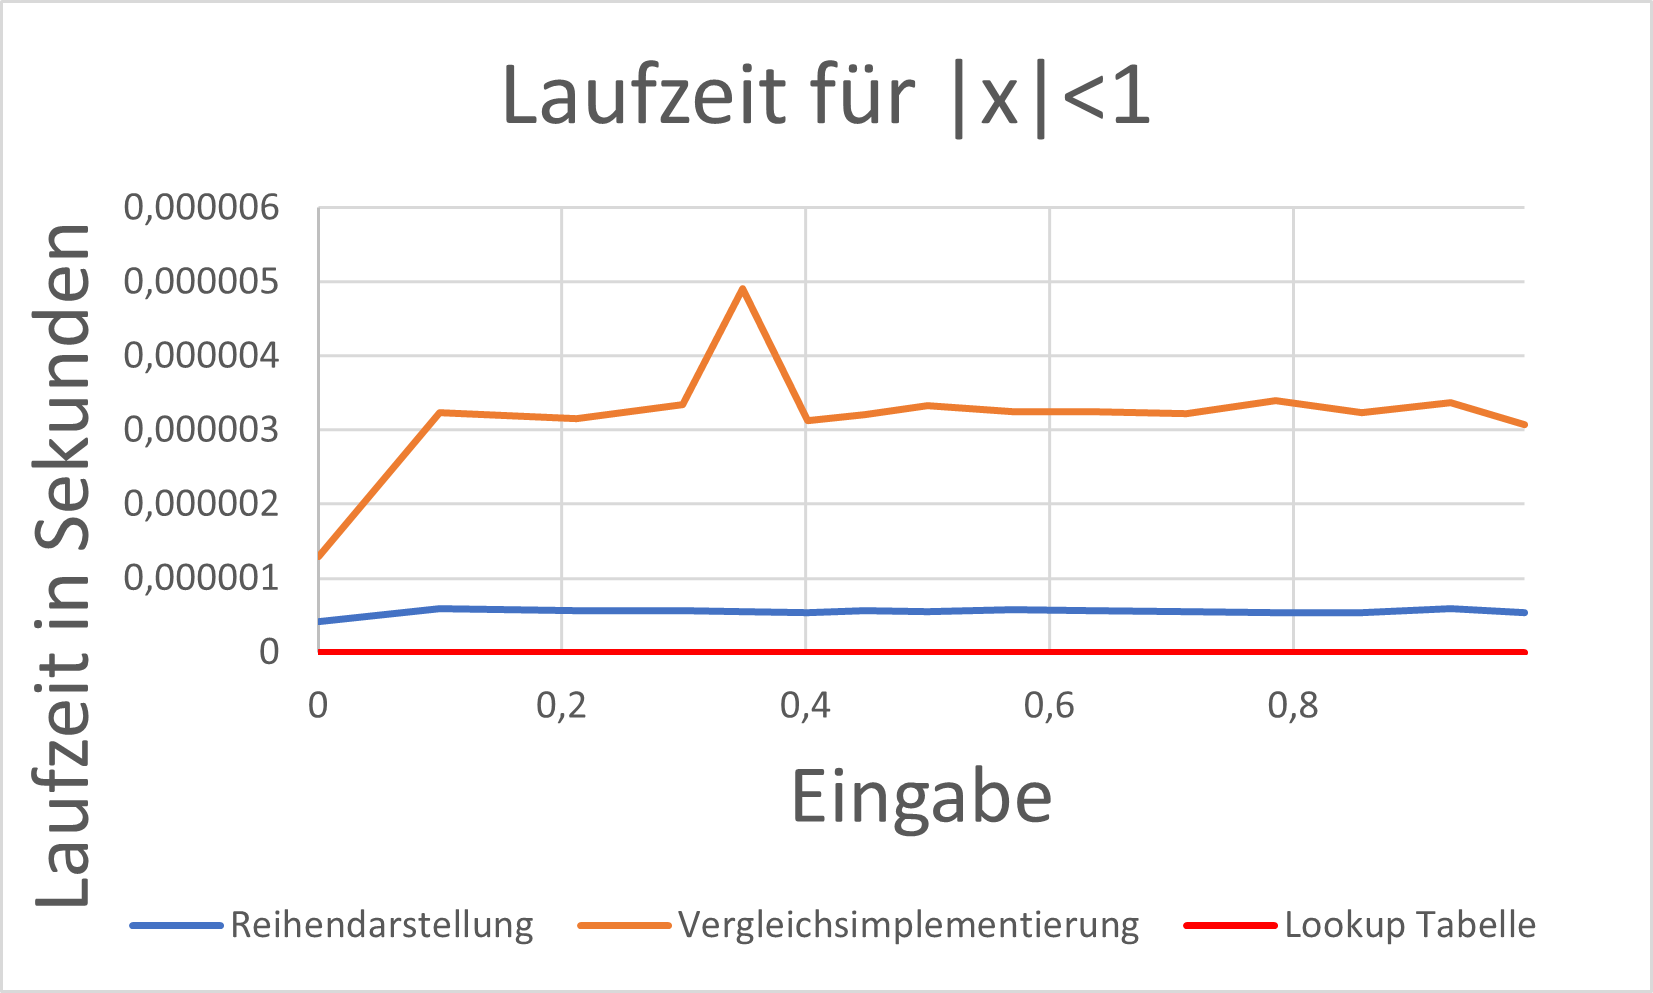
\includegraphics[width=0.49\textwidth]{newnewLaufzeit1.png}
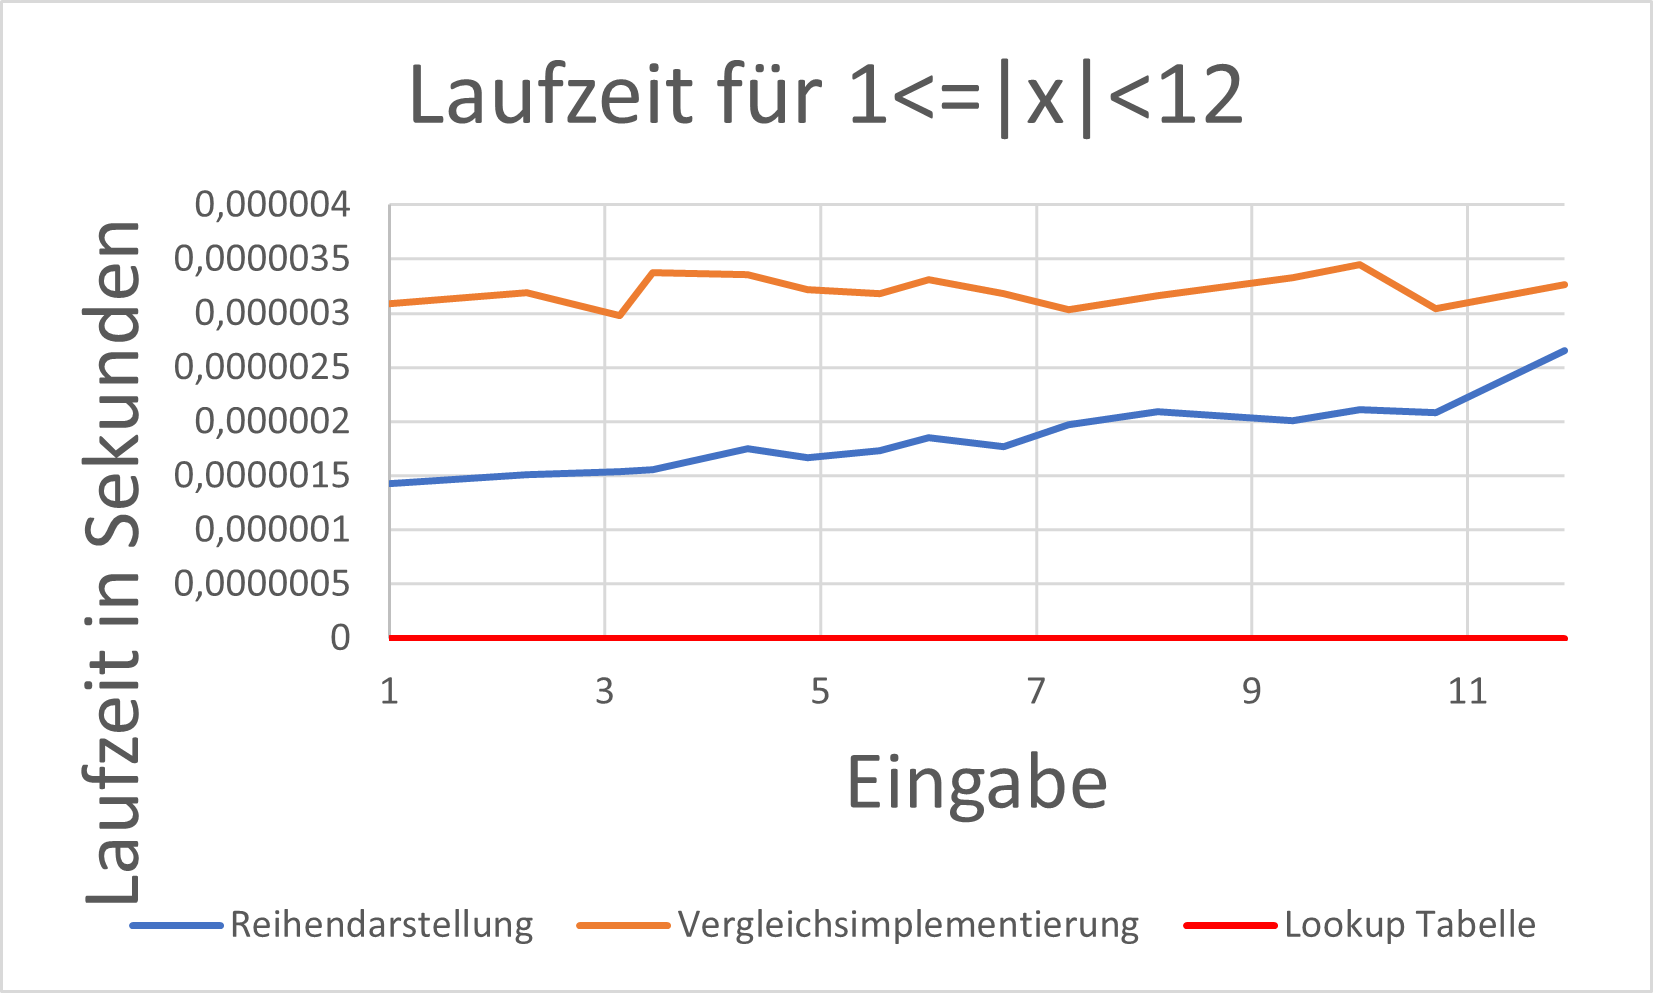
\includegraphics[width=0.49\textwidth]{newnewLaufzeit2.png}
\end{figure}

\begin{figure}
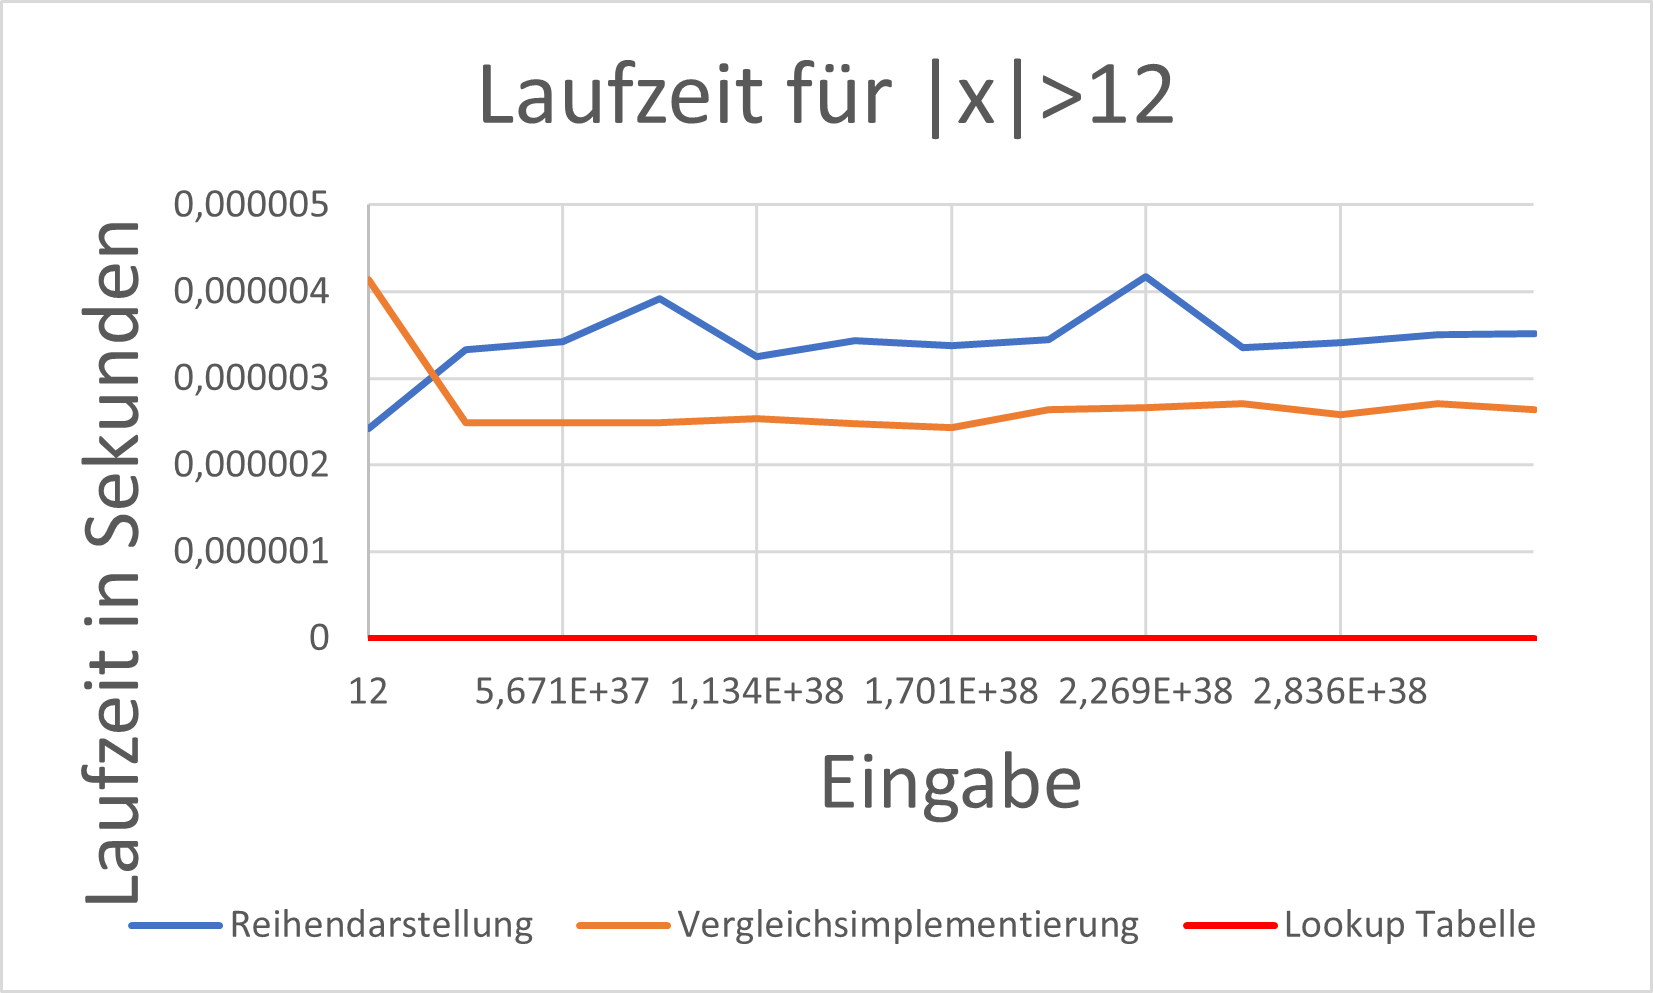
\includegraphics[width=0.49\textwidth]{Laufzeitnewnew3.png}
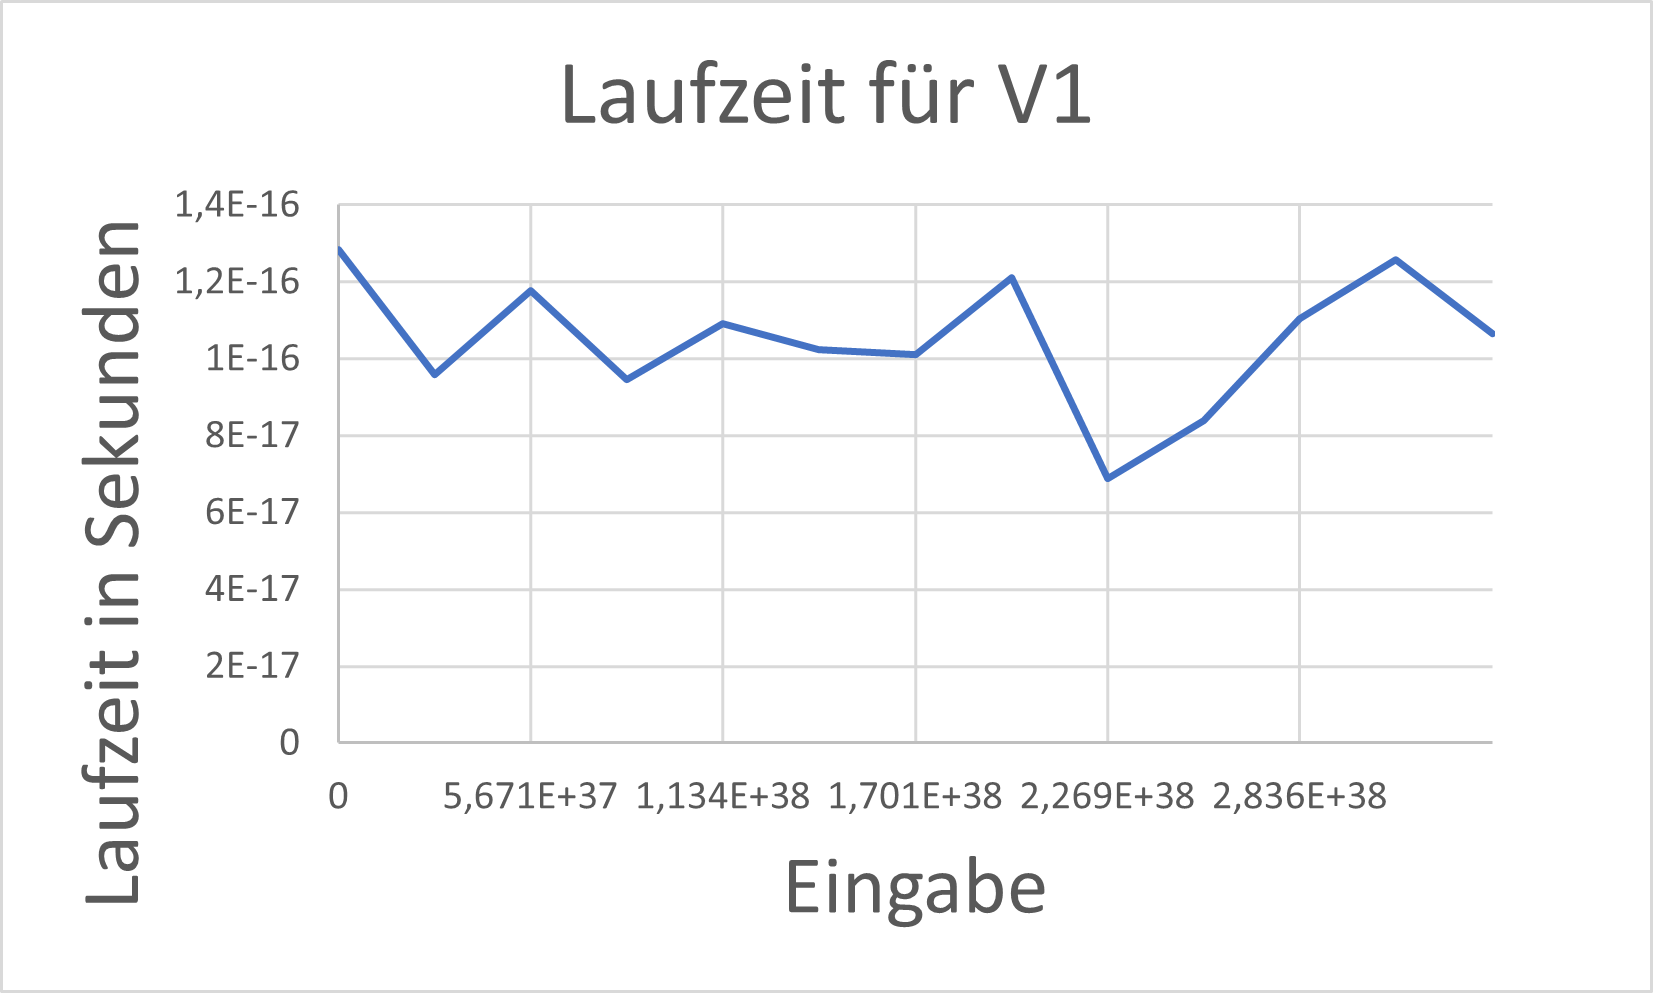
\includegraphics[width=0.49\textwidth]{Laufzeitlookup.png}
\end{figure}

Zum Vergleich wurde auch die $CPU \ Time$ anhand von drei Eingabewerten aus den drei zuvor beschriebenen Definitionsbereichen analysiert. 
Für $x=0.5$ liegt die $CPU \ Time$ für V0 bei $5.97e-7$, für V1 bei $1.2270e-15$ und für V2 bei $4.479e-6$, während die Laufzeit von $CLOCK\_MONOTONIC\_RAW$ für V0 bei $5.44e-7$ für V1 bei $1.132e-16$ und für V2 bei $3.204e-6$.
Für $x=6.7$ ist die Laufzeit für V0 $1.982e-6$, für V1 $9.923\epsilon-16$ und für V2 $3.602e-6$ bei der Analyse durch $CPU \ Time$. $CLOCK\_MONOTONIC\_RAW$ gibt dann für V0 $1.769e-6$, für V1 $9.83e-17$ und für V2 $3.182e-6$ zurück. Der Wert $x=1.701411735e+38$ wird dann durch $Clock \ Time$ für V0 $3.387e-6$, für V1 $1.1055e-15$ und für V2 $2.797e-6$ zurückgegeben. Des Weiteren bei  $CLOCK\_MONOTONIC\_RAW$ wird für V0 $3.376e-6$, für V1 $1.01e-16$ und für V2 $2.433e-6$ ausgegeben.

$CLOCK\_MONOTONIC$ ist also für alle Implementierungen und Eingabewerte schneller als $CPU \ Time$. Dies kann daran liegen, dass $CPU \ Time$ lediglich über einen Prozessorkern arbeitet und dass innerhalb der für die Laufzeit relevanten Bereiche der Implementierungen keine I/O Befehle verwendet werden, welche die Laufzeit von $CLOCK\_MONOTONIC\_RAW$ beeinträchtigen würden.
 
 \section{Zusammenfassung und Ausblick}
 
 Im Rahmen des Projektes zum Thema der Approximation der Areasinus Hyperbolicus Funktion (arsinh), der Umkehrfunktion des Sinus Hyperbolicus (sinh) und der Analyse der implementierten Berechnungen wurde anhand der bestimmten Lösungsansätze die dafür zuständigen Implementierungen umgesetzt, deren Ausführung durch das Rahmenprogramm erfolgte, welches die Nutzung der unterschiedlichen Implementierungen sowie Laufzeitberechnungen ermöglichte.   
 
 Die Implementierung mit der Reihendarstellung kam dank der durchgeführten Umformungen, wie z.B. mit Taylorreihe oder binomischer Reihe, zustande. Die Idee bei der Implementierung mit den Suchtabellen wurde mit der Verwendung von linearer Interpolation realisiert, wobei es zuerst eine Wahl zwischen den unterschiedlichen Interpolationen durchlief. Mit diesen Ansätzen wurde die Grundstruktur vom umgesetzten Programm aufgebaut. Im Weiteren ging es um die genauere Approximation und performantere Implementierung. Dies ließ sich im Verhältnis mit einer Vergleichsimplementierung einschätzen. Dabei wurden nicht nur die berechneten Werte, sondern auch die gemessenen Laufzeiten verglichen.  
 
 Zusammenfassend lässt sich anhand der implementierten und zu analysierenden Berechnungen schlussfolgern, dass die Approximation der Funktion Areasinus Hyperbolicus  sich mit der Reihendarstellung genauer bestimmen lässt und zu alledem mit der Nutzung von ausschließlich einfachen Operationen für kleinere Eingabewerte performanter als die Vergleichsimplementierung ist. Allerdings besteht ein wesentlicher Unterschied zur LookUp-Tabellen Methode, welche um ein Vielfaches performanter als die Reihendarstellung ist, aber eine geringere Genauigkeit nachweist, weil sie mehr Speicherplatz für mehrere Tabellen zur Genauigkeitserhöhung benötigt.
 
 Eine unterschiedliche Vorgehensweise zur Implementierung von V0 und V1 wäre es, ein Array von Eingabewerten zu erwarten, dass über SIMD Befehle verarbeitet wird.
 
 % TODO: Fuegen Sie Ihre Quellen der Datei Ausarbeitung.bib hinzu
 % Referenzieren Sie diese dann mit \cite{}.
 % Beispiel: CR2 ist ein Register der x86-Architektur~\cite{intel2017man}.
 \bibliographystyle{plain}
 
 \bibliography{bibliography.bib}{}
 \end{document}